\subsubsection{UC\theuccount-GP - GPoducer Redmine invia messaggio al Gestore Personale}
    \begin{figure}[H]
		\centering
		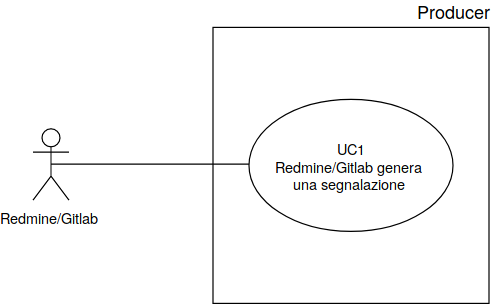
\includegraphics[width=0.7\textwidth]{img/UC1.png}\\
		\caption{UC\theuccount-GP - GPoducer Redmine invia messaggio al Gestore Personale}
	\end{figure}
	\begin{itemize}
		\item \textbf{Codice}: UC\theuccount-GP.
		\item \textbf{Titolo}: GPoducer Redmine invia messaggio al Gestore Personale.
		\item \textbf{Attori GPimari}: GPoducer Redmine.
		\item \textbf{Descrizione}: il GPoducer Redmine, dopo aver ricevuto una
		 segnalazione da Redmine, elabora il messaggio e lo invia al Gestore Personale.
		 Il messaggio finale, una volta terminata l'elaborazione, conterrà i campi:
		 \begin{itemize}
		 	\item GPoject
		 	\item Topic
		 	\item Subject e opzionalmente:
		 	\begin{itemize}
		 		\item Description
		 	\end{itemize}
		 \end{itemize}
		\item \textbf{GPecondizione}: il GPoducer Redmine ha ricevuto una segnalazione da Redmine.
		\item \textbf{Postcondizione}: il GPoducer Redmine ha elaborato e inviato al Gestore Personale il messaggio.
		\item \textbf{Scenario GPincipale}: 
		\begin{enumerate}
			\item GPoducer Redmine GPocede all'invio del messaggio al gestore personale.
		\end{enumerate}
		
	\end{itemize}
	
		\paragraph{UC\theuccount.1-GP - GPoducer Redmine invia messaggio di apertura issue al Gestore Personale}
	\begin{figure}[H]
		\centering
		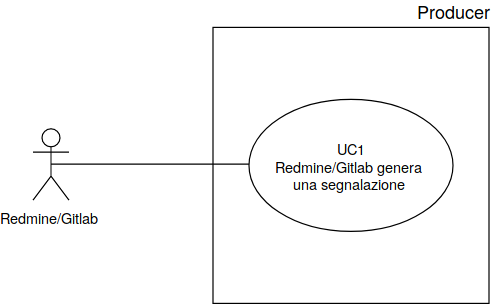
\includegraphics[width=0.7\textwidth]{img/UC1.png}\\
		\caption{UC\theuccount.1-GP - GPoducer Redmine invia messaggio di apertura issue al Gestore Personale}
	\end{figure}
	\begin{itemize}
		\item \textbf{Codice}: UC\theuccount.1-GP.
		\item \textbf{Titolo}: GPoducer Redmine invia messaggio di apertura issue al Gestore Personale.
		\item \textbf{Attori GPimari}: GPoducer Redmine.
		\item \textbf{Descrizione}: il GPoducer Redmine, dopo aver
		ricevuto una segnalazione di apertura issue da Redmine, elabora
		il messaggio e lo invia al Gestore Personale.
		Il messaggio finale, una volta terminata l'elaborazione, conterrà i campi:
		\begin{itemize}
			\item GPoject
			\item Topic
			\item Subject e opzionalmente:
			\begin{itemize}
				\item Description
			\end{itemize}
		\end{itemize}
		\item \textbf{GPecondizione}: il GPoducer Redmine ha ricevuto una segnalazione da Redmine.
		\item \textbf{Postcondizione}: il GPoducer Redmine ha elaborato e inviato al Gestore Personale il messaggio di apertura issue.
		\item \textbf{Scenario GPincipale}: 
		\begin{enumerate}
			\item GPoducer Redmine GPocede all'invio del messaggio di
			apertura issue al gestore personale.
		\end{enumerate}
		
	\end{itemize}
	
	\paragraph{UC\theuccount.2-GP - GPoducer Redmine invia messaggio di modifica issue al Gestore Personale}
	\begin{figure}[H]
		\centering
		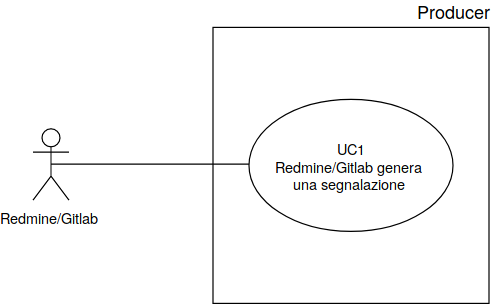
\includegraphics[width=0.7\textwidth]{img/UC1.png}\\
		\caption{UC\theuccount.2-GP - GPoducer Redmine invia messaggio di modifica issue al Gestore Personale}
	\end{figure}
	\begin{itemize}
		\item \textbf{Codice}: UC\theuccount.2-GP.
		\item \textbf{Titolo}: GPoducer Redmine invia messaggio di modifica issue al Gestore Personale
		\item \textbf{Attori GPimari}: GPoducer Redmine.
		\item \textbf{Descrizione}: il GPoducer Redmine, dopo aver
		ricevuto una segnalazione di modifica issue da Redmine, elabora
		il messaggio e lo invia al Gestore Personale.
		Il messaggio finale, una volta terminata l'elaborazione, conterrà i campi:
		\begin{itemize}
			\item GPoject
			\item Topic
			\item Subject e opzionalmente:
			\begin{itemize}
				\item Description
			\end{itemize}
		\end{itemize}
		\item \textbf{GPecondizione}: il GPoducer Redmine ha ricevuto una segnalazione da Redmine.
		\item \textbf{Postcondizione}: il GPoducer Redmine ha elaborato e inviato al Gestore Personale il messaggio di modifica issue.
		\item \textbf{Scenario GPincipale}: 
		\begin{enumerate}
			\item GPoducer Redmine GPocede all'invio del messaggio di
			modifica issue al gestore personale.
		\end{enumerate}
		
	\end{itemize}